\documentclass[tc, manuscript]{copernicus}

\usepackage{booktabs}
\usepackage{multirow}
\usepackage{siunitx} 

\begin{document}

\title{Improving water-use efficiency of artificial ice reservoirs (Icestupas) through weather-sensitive fountain scheduling
strategies}

\def\Authors{Suryanarayanan Balasubramanian\,$^{1,2}$, Martin Hoelzle\,$^{1}$Roger Waser\,$^{3}$}

\def\Address{$^{1}$University of Fribourg, Department of Geosciences, Fribourg, Switzerland $^{2}$University of
Applied Sciences and Arts, Luzern, Switzerland} \def\corrAuthor{Suryanarayanan Balasubramanian}
\Author[1,2]{Suryanarayanan}{Balasubramanian}
\Author[1]{Martin}{Hoelzle}
\Author[3]{Roger}{Waser}
% \Author[3]{Martin}{Von Burg}
\affil[1]{University of Fribourg, Department of Geosciences, Fribourg, Switzerland}
\affil[2]{Himalayan Institute of Alternatives, Ladakh, India}
\affil[3]{University of Applied Sciences and Arts, Luzern, Switzerland}

\correspondence{suryanarayanan.balasubramanian@unifr.ch}

\runningtitle{Scheduling AIR fountains}

\runningauthor{S. Balasubramanian}

\firstpage{1}

\maketitle

\begin{abstract}

  Artificial Ice Reservoirs (AIRs), often also called - Ice Stupas - are a climate change adaptation strategy
  developed in the Indian Himalayas (Ladakh). With this technology, otherwise unused stream water is stored in
  large ice towers in winter. The surplus melt water that is generated in spring is used for satisfying
  irrigation water demands. Recent studies have shown that during construction of traditional AIRs over 75 \% of
  the water sprayed was lost. Therefore, fountain wastewater production has to be reduced for improving water
  use efficiency.  During the winter of 2021-22, a traditional and an automated AIR were built in Guttannen,
  Canton of Berne, Switzerland with the main aim of comparing and quantifying the benefits of fountain
  scheduling. Fountain scheduling was realized through an automation system computing recommended discharge
  rates using real-time weather input and location metadata. The scheduled fountain produced similar volumes
  while consuming 87 \% less water than the unscheduled fountain. Simulations converting unscheduled fountains
  to scheduled fountains improved the water use efficiency of several traditional AIRs more than two fold.
  Overall, these results show that the automated construction strategy can increase the water use efficiency of
  AIRs without compromising their meltwater production.

\end{abstract}

\introduction

Cryosphere-fed irrigation networks in arid mountain regions are completely dependent on timely availability of
meltwater from glaciers, snow and permafrost \citep{immerzeelImportanceVulnerabilityWorld2020, farhanHydrologicalRegimesConjunction2015,
tveitenGlacierGrowingLocal2007}. With the accelerated decline of glaciers due to climate change
\citep{nusserLocalKnowledgeGlobal2016}, these regions are experiencing water scarcity particularly during the
spring season \citep{norphelSnowWaterHarvesting2015}. This seasonal water scarcity makes it essential to provide
supplementary irrigation in order to sustain agricultural output and take advantage of the complete growing
season \citep{nusserLocalKnowledgeGlobal2016, vincentEnergyClimateChange2009}.

To cope with this recurrent water scarcity, villagers in the region of Ladakh have developed two types of
artificial ice reservoirs (AIRs): horizontal and vertical (see Fig. \ref{fig:AIRforms}).  All these types of ice
reservoirs capture water in the autumn and winter, allowing it to freeze, and hold it until spring, when it
melts and flows down to fields \citep{ipccChapterHighMountain2019, vinceGlacierMan2009,
clouseLadakhArtificialGlaciers2017, nusserSociohydrologyArtificialGlaciers2019}. In this way, they retain a
previously unused portion of the annual flow and facilitate its use to supplement the decreased flow in the
following spring. This study focuses on the vertical form of AIRs locally called as ice stupas.

\begin{figure}[t]
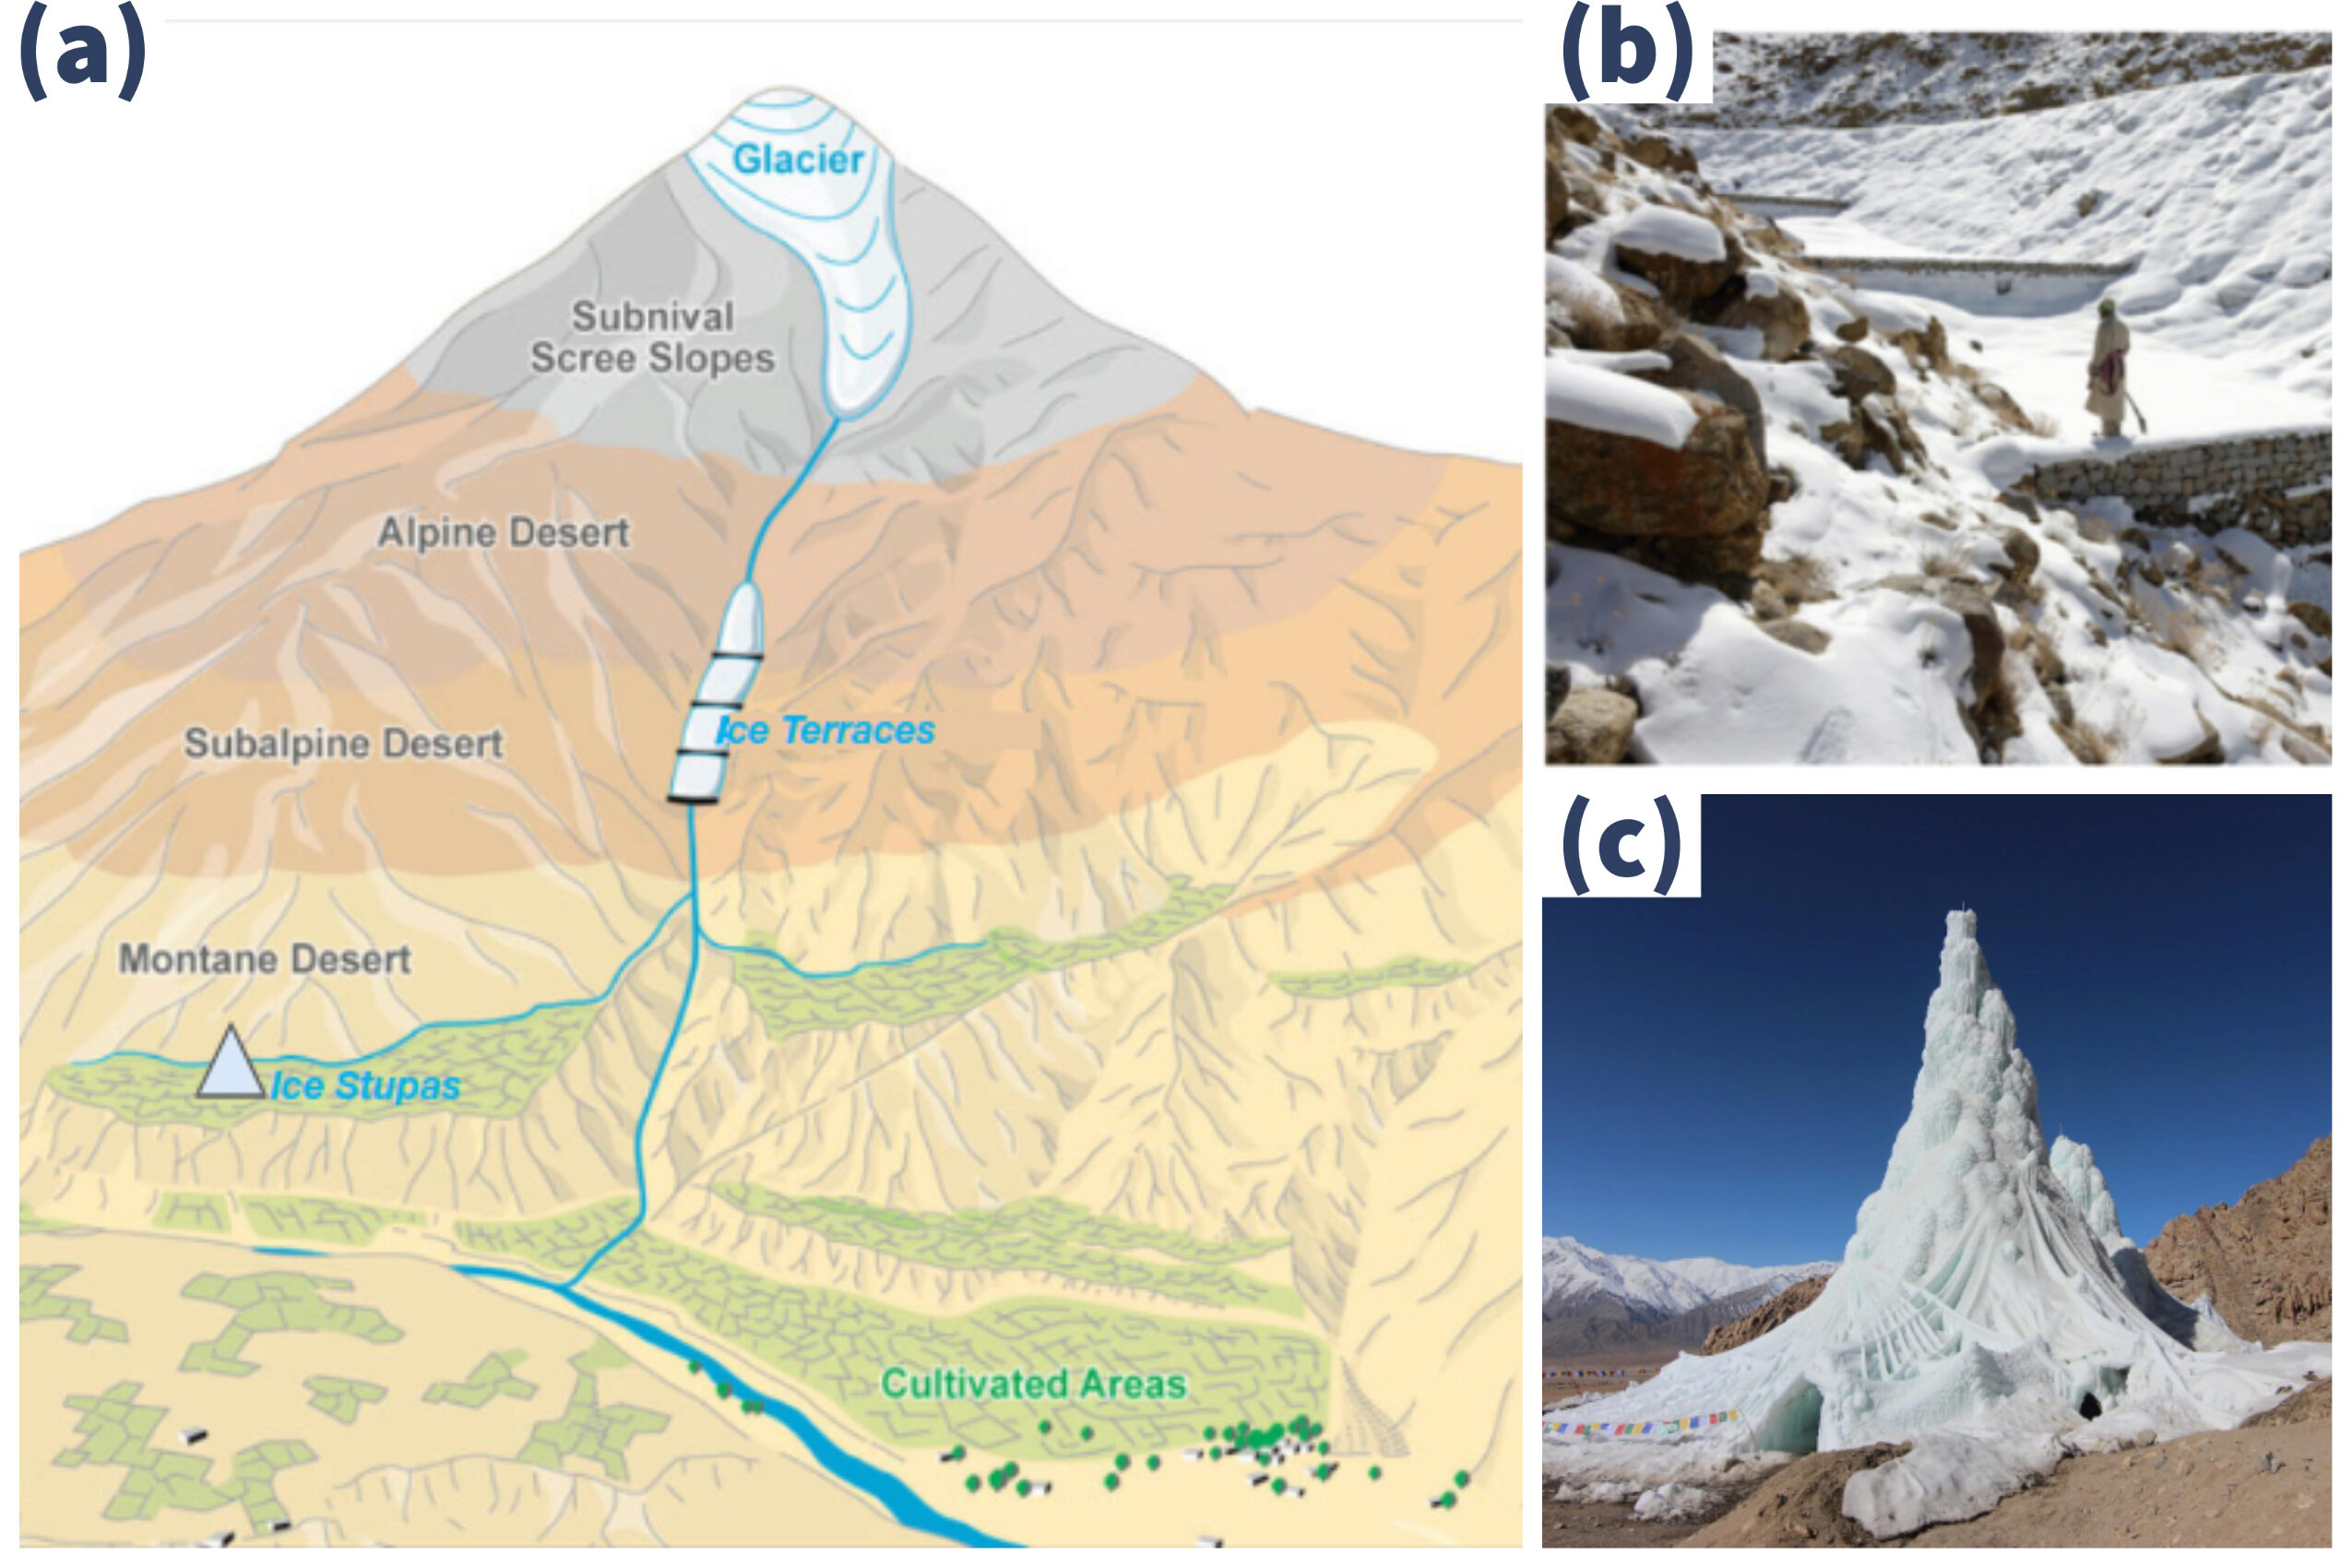
\includegraphics[width=12cm]{Figures/AIR_forms.jpg}

\caption{(a) Schematic overview of the position of artificial ice reservoirs. These constructions are located at
altitudes between the glaciers and the irrigation networks in the cultivated areas. Horizontal and vertical AIRs
are located at higher and lower altitudes respectively. Adapted from: \cite{nusserLocalKnowledgeGlobal2016}}

\label{fig:AIRforms}
\end{figure}

Over the past decade, several ice stupas have been built to supplement irrigation water supply of mountain
villages in India \citep{wangchukIceStupaCompetition2020, palmerStoringFrozenWater2022,
aggarwalAdaptationClimateChange2021}, Kyrgyzstan \citep{bbcnewsBrightArtificialGlacier2020} and Chile
\citep{reutersConservationistsChileAim2021}. These AIRs are traditionally constructed by diverting springs or
glacial streams into fountain spray systems via embankments and pipelines. 

One of the most common problems with AIR construction systems has to do with fountain scheduling. Fountain
scheduling is simply answering the questions of “When do I spray?” and “How long do I spray?”. Starting fountain
spray too early and/or running a fountain spray too long is considered over watering. At the very least this
practice wastes water. However, overwatering can cause accelerated ice melt if done on a prolonged basis.
Likewise, starting fountain spray too late or not running the system for a long enough period of time is
considered under watering and can cause reduced ice volumes.

Previous work \citep{balasubramanianInfluenceMeteorologicalConditions2022} has shown that traditional
construction systems tend to suffer from overwatering. Knowledge of surface freezing rates is important to
avoid overwatering. Surface freezing rates can be calculated by means of the full energy balance model
developed in \cite{balasubramanianInfluenceMeteorologicalConditions2022}. This model can be forced with either
historical weather data or real-time weather data to produce recommended discharge rates.

However, there are several issues that need to be addressed before operating such weather-sensitive fountains.
For example, in the case of the Indian AIR, the fountain discharge rate could have been halved since they were
always two times higher than the modelled freezing rate
\citep{balasubramanianInfluenceMeteorologicalConditions2022}. However, in practice, reduction of discharge rate
would compromise the maximum ice volume obtained due to reduction in the fountain spray radius and could
increase the maintenance cost due to higher risk of fountain freezing events.  

An optimum construction strategy, therefore, should first prevent the occurence of these two events before
reducing discharge rates. Spray radius can be maintained if the fountain aperture diameter is lowered with the
discharge rate. Fountain freezing events can be prevented if the discharge is not lowered below a minimum
threshold. 

Recommended discharge rate needs to be sensitive to constraints on the water supply or weather of the
construction site. Locations limited by their water supply like in Ladakh, India would prioritize water use
efficiency whereas those limited by the favourable weather windows like in Guttannen, Switzerland  would
prioritize for maximum ice volume.  Accordingly, we use two types of model parameter forcings that prevent
underwatering and overwatering to attain higher ice volumes and higher water use efficiency respectively. 

However, manually adjusting the fountain discharge rate is not practical due to two reasons. Firstly, this would
involve constant adjustments of discharge rates in response to the significant diurnal and seasonal variations
of the freezing rates. Secondly, frequent pipeline water drainage is required to avoid water losses. Therefore,
operation of weather-sensitive fountains via automation systems is preferred to reduce the maintenance cost
long-term.

The present study was performed to compare two AIRs produced using different fountain scheduling strategies but
exposed to identical meteorological conditions. The specific objectives of this paper include the water-use
efficiency and maximum ice volume comparison of different fountain scheduling strategies, presentation of the
automation system, and examples of its application to the computation of fountain scheduling strategies.

\section{Study sites and data}

In this study, we use some datasets presented in our previous work
\citep{balasubramanianInfluenceMeteorologicalConditions2022} along with new datasets. These old datasets record
the meteorological conditions and fountain characteristics of AIRs built in Gangles, India (IN21) and Guttannen,
Switzerland (CH21) during the winter of 2020-21. In this section, we focus on describing the AIR datasets
collected in Guttannen, Switzerland during the winter of 2021-22 (CH22).

The Guttannen site (46.66 $\degree$N, 8.29 $\degree$E) is situated in the Berne region, Switzerland and has an
altitude of 1047 $m$ a.s.l. In the winter (Oct-Apr), mean daily minimum and maximum air temperatures vary
between -13 and 15 $\degree C$. Clear skies are rare, averaging around 7 days during winter. Daily winter
precipitation can sometimes be as high as 100 $mm$. These values are based on 30 years of hourly historical
weather data measurements \citep{meteoblueClimateGuttannen2021}. Two AIRs were constructed by the Guttannen
Bewegt Association, the University of Fribourg and the Lucerne University of Applied Sciences and Arts during
the winters of 2021-22 using a traditional and an automated construction strategy.

\begin{figure}[t]
\includegraphics[width=12cm]{Figures/2AIRs.jpg}
\caption{Automated and traditional AIRs at Guttannen on February 6, 2022. Picture credits: Daniel Bürki}
\label{fig:2AIR}
\end{figure}

The automated and the traditional AIRs were constructed adjacent to each other as shown in Fig. \ref{fig:2AIR}.
This ensured both AIRs shared the same water source and identical weather conditions. In addition, a webcam
guaranteed a continuous survey of the automated AIR.   

In the traditional strategy, the fountain was operated manually whereas in the automated strategy a programmed
automation system controlled the fountain discharge rate during the whole study period using real time weather
input and several control parameters, which could be modified via a user interface. Henceforth, we refer to the
fountain used in the traditional and automated construction strategy as unscheduled and scheduled fountains
respectively.

In the traditional construction strategy, tree branches were laid covering the fountain pipe to initiate and
speed up the ice cone formation process. In the automated strategy, only the fountain pipe was placed before the
water spray started. The construction of both the AIRs began on 8th December on a snow bed of 13 cm thickness
and ended on 12th April. These two dates are denoted as start and expiry dates henceforth.

\subsection{Meteorological data}

Air temperature, relative humidity, wind speed, pressure, long-wave, short-wave direct and diffuse radiation are
required to calculate the surface energy balance of an AIR.  The weather data source was an automatic weather
station (AWS) located around 20 m away as shown in Fig. \ref{fig:2AIR}. Less than 0.4 \% of the data was found
to be missing and the data gaps were filled by linear interpolation. Hourly ground temperature measurements were
also recorded by the AWS to approximate the fountain's water temperature. 

\begin{figure*}[t]
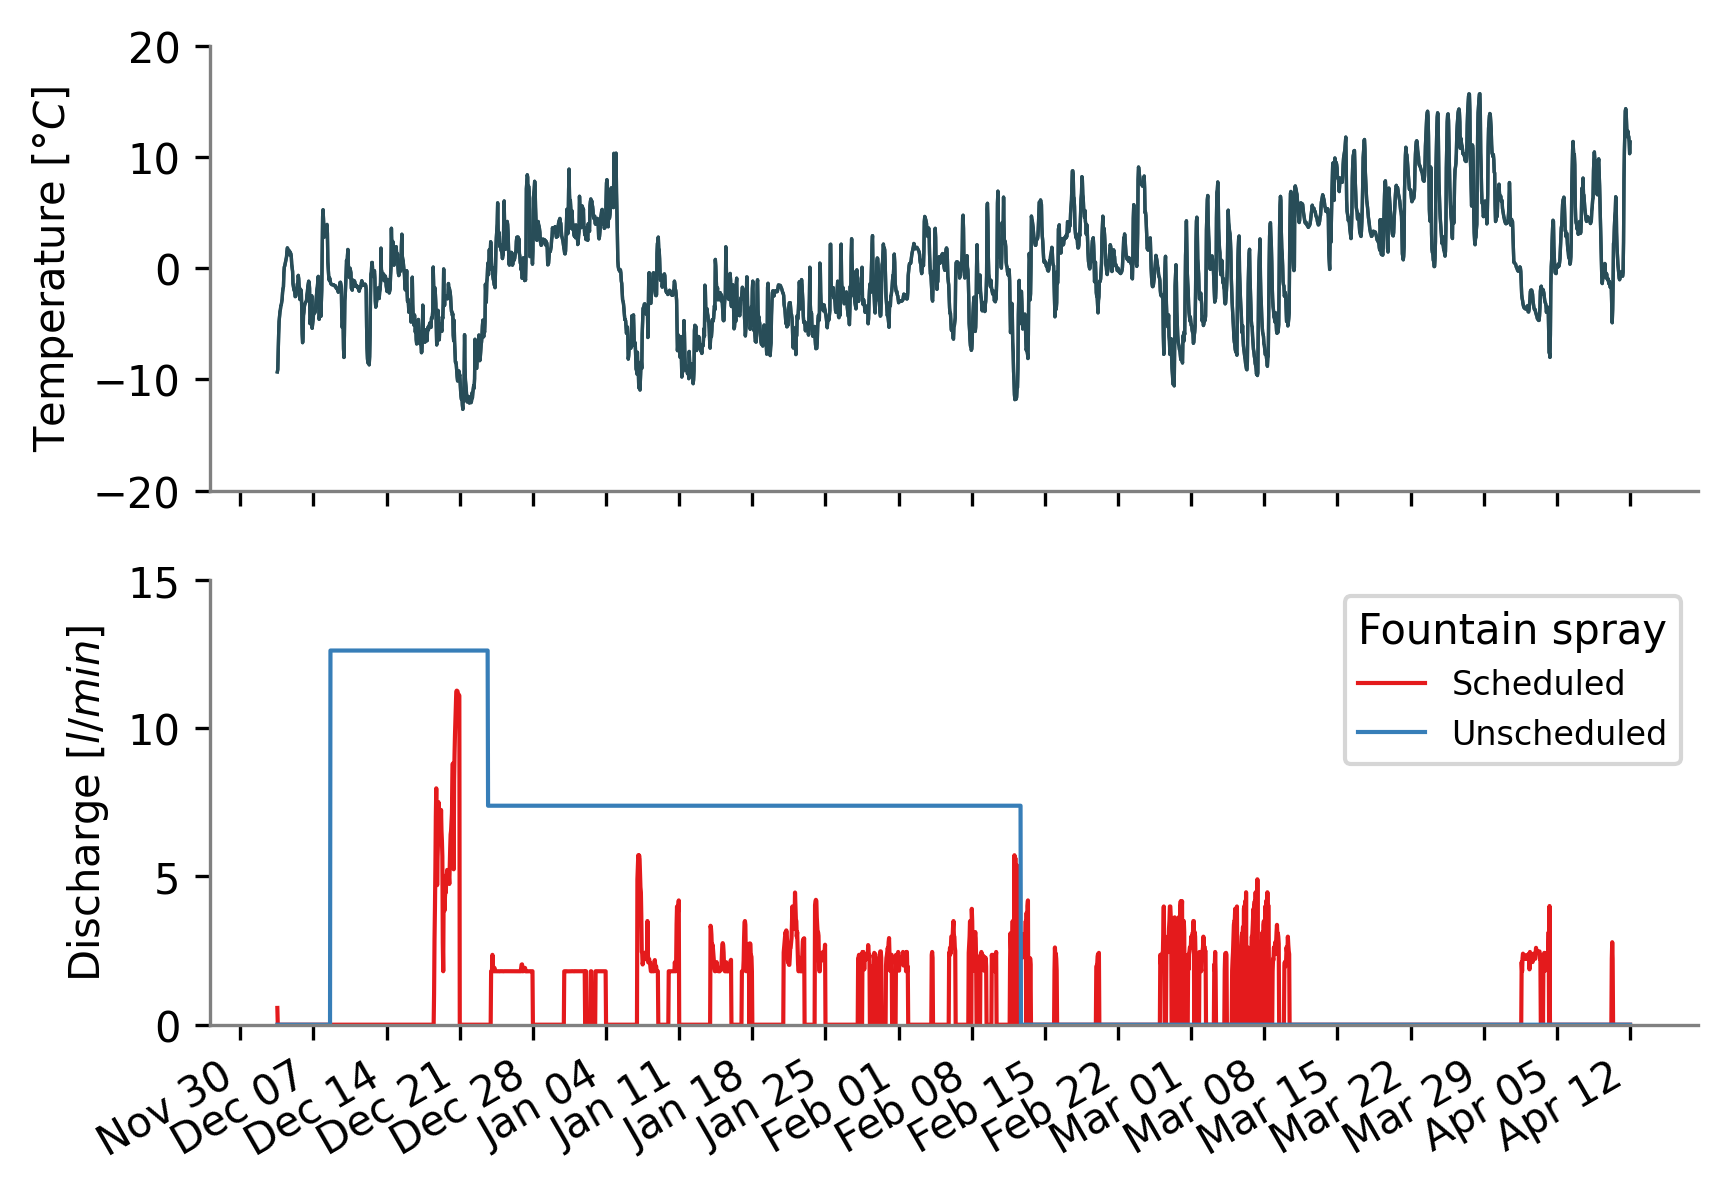
\includegraphics[width=12cm]{Figures/disvstemp.png}
\caption{Temperature and discharge measurements at the Guttannen construction site}
\label{fig:aws} 
\end{figure*}


\subsection{Fountain observations}

The fountain consists of a pipeline and a nozzle. The pipeline has three attributes, namely : discharge rate
($Q$), height ($h$) and water temperature ($T_F$). Discharge rate represents the discharge rate of the water in
the fountain pipeline. Height denotes the height of the fountain pipeline installed. Fountain water temperature
is the temperature of water droplets produced by the fountain.

The fountain nozzle has three characteristics, namely : the aperture diameter ($dia$), the spray radius ($r$)
and pressure loss ($P$) .The fountain nozzle is assumed to have only one aperture with diameter $dia$ from where
water is sprayed. Spray radius denotes the observed ice radius formed from the fountain water droplets.
Pressure loss denotes the loss of water head caused due to the fountain nozzle.

Fig. \ref{fig:aws} shows how the automation system scheduled the discharge rate based on real-time
meteorological conditions. The automation system caused these variations through its control valve which varied
between 0 to 100 \% depending on the recommended discharge rate. Throughout the study period, the control valve
was opened completely (100 \%) only once corresponding to the time when the temperature attained its minimum of
-13 \degree C on 20th December. After this event, the control valve was never opened beyond 34 \%.  

The unscheduled fountain was manually operated to spray all the available discharge until a fountain freezing
event interrupted the discharge on 17th February. Unfortunately, no discharge rate measurements were recorded
for the unscheduled fountain. Therefore, this dataset was estimated from the discharge rate measurements and
characteristics of the scheduled fountain.

The height was also increased in steps of 1 meter for both the fountains. This caused variations in the
corresponding discharge rate. For the scheduled fountain, the construction began with a height of 3 m with an
increase to 4 $m$ on 23rd December. This fountain height increase reduced its maximum discharge from
13 $l/min$ to 11 $l/min$. For the unscheduled fountain, the construction began with a height of 3.7 $m$ and then
this was increased two times on 23rd December and 12th February.  

The water temperature of both the fountains were estimated from the AWS ground temperature dataset.

The spray radius was estimated for both the fountains from several drone flights. Ice radius measurements of
drone flights which observed either an increase in AIR circumference or volume were averaged to determine the
fountain's spray radius.

\subsection{Drone surveys}

Several photogrammetric surveys were conducted on the traditional and the automated AIRs. The details of these
surveys and the methodology used to produce the corresponding outputs are explained in
\cite{balasubramanianInfluenceMeteorologicalConditions2022}. The digital elevation models (DEMs) generated from
the obtained imagery were analysed to document the spray radius, the surface area and the volume of the ice
structures.  The number of drone surveys conducted for the traditional and the automated AIRs were 8 and 6,
respectively (see Table \ref{tab:uav}). 

\begin{table}
	\centering
	\caption{ Summary of the drone surveys}
	\label{tab:uav}
	\begin{tabular}{@{}|llllll|@{}}
		\toprule
		\textbf{}              & \textbf{No.} & \textbf{Date} & \textbf{Volume} & \textbf{Radius} & \textbf{Surface Area} \\ \midrule
		\multicolumn{1}{|l|}{\multirow{8}{*}{\rotatebox[origin=c]{90}{Traditional}}}
		                       & 1            & Dec 23, 2021  & 17 $m^{3}$     & 2.9 $m$
		                       & 47 $m^{2}$                                                                      \\
		\multicolumn{1}{|l|}{} & 2            & Jan 3, 2022  & 22 $m^{3}$     & 3.4 $m$
		                       & 61 $m^{2}$                                                                      \\
		\multicolumn{1}{|l|}{} & 3            & Jan 22, 2022   & 35 $m^{3}$     & 4 $m$
		                       & 79 $m^{2}$                                                                      \\
		\multicolumn{1}{|l|}{} & 4            & Feb 6, 2022  & 44 $m^{3}$     & 4.2 $m$
		                       & 86 $m^{2}$                                                                      \\
		\multicolumn{1}{|l|}{} & 5            & Feb 20, 2022  & 43 $m^{3}$     & 4.3 $m$
		                       & 86 $m^{2}$                                                                      \\
		\multicolumn{1}{|l|}{} & 6            & Mar 19, 2022  & 33 $m^{3}$     & 4.4 $m$
		                       & 84 $m^{2}$                                                                      \\
		\multicolumn{1}{|l|}{} & 7            & Mar 26, 2022  & 24 $m^{3}$     & 4.3 $m$
		                       & 74 $m^{2}$                                                                      \\
		\multicolumn{1}{|l|}{} & 8            & Apr 12, 2022  & 11 $m^{3}$     & 3.5 $m$
		                       & 50 $m^{2}$                                                                      
		\\\midrule
		\multicolumn{1}{|l|}{\multirow{6}{*}{\rotatebox[origin=c]{90}{Automated}}}
		                       & 1            & Dec 23, 2021  & 35 $m^{3}$      & 4.3 $m$
		                       & 73 $m^{2}$                                                                       \\
		\multicolumn{1}{|l|}{} & 2            & Jan 3, 2022   & 32 $m^{3}$      & 4.4 $m$
		                       & 81 $m^{2}$                                                                       \\
		\multicolumn{1}{|l|}{} & 3            & Feb 20, 2022   & 60 $m^{3}$      & 5.3 $m$
		                       & 105 $m^{2}$                                                                       \\
		\multicolumn{1}{|l|}{} & 4            & Mar 19, 2022   & 28 $m^{3}$      & 3.7 $m$
		                       & 57 $m^{2}$                                                                       \\
		\multicolumn{1}{|l|}{} & 5            & Mar 26, 2022   & 19 $m^{3}$      & 3.7 $m$
		                       & 53 $m^{2}$                                                                       \\
		\multicolumn{1}{|l|}{} & 6            & Apr 12, 2022   & 7 $m^{3}$      & 2.5 $m$
		                       & 53 $m^{2}$                                                                       \\
		\bottomrule
	\end{tabular}

\end{table}

\section{Methods}

\subsection{Automation system}

Any construction location can either be constrained by the available water supply or the duration of favourable
weather windows for fountain operation. If the respective location has limited water supply then the fountain
scheduling strategy should be optimised for water-use efficiency . But if the location is limited by the time
period when the fountain can function then the scheduling strategy should be optimised for ice volumes.

Accordingly, we introduce two kinds of model forcing assumptions corresponding to the ice volume and water-use
efficiency objective for the following three model variables: (a) slope , (b) albedo and (c) cloudiness.   The
slope variable increases the shortwave radiation and sensible heat impact. The albedo variable decreases the
shortwave radiation impact. The cloudiness variable increases both the shortwave and the longwave radiation
impact. Therefore, increase of slope and cloudiness variable increases melting energy and increase of albedo
variable increases freezing energy. Assumptions used for the ice volume and water-use efficiency objectives
overestimate and underestimate the freezing rate of the AIR respectively. Correspondingly, we associate the
upper and lower bounds of these variables as shown in Table \ref{tab:assumptions}. These two kinds of models
will be referred to as model optimised for ice volume (MIV) and model optimised for water-use efficiency (MWE)
respectively. 

\begin{table}[]
\centering
\caption{Assumptions for the parametrisation introduced to simplify the model.}
\label{tab:assumptions}
\begin{tabular}{@{}lllll@{}}
\toprule
\textbf{Estimation of} & \textbf{Symbol} & \textbf{MIV} & \textbf{MWE} & \\ \midrule
\multicolumn{1}{|l}{Slope}        & $s_{cone}$ & $ 1 $ & $0$ & \multicolumn{1}{l|}{} \\ \midrule
\multicolumn{1}{|l}{Albedo} & $\alpha$ & $\alpha_{snow}$ & $\alpha_{ice}$ & \multicolumn{1}{l|}{} \\\midrule 
\multicolumn{1}{|l}{Cloudiness}  & $cld$ & $0$ & $1$ & \multicolumn{1}{l|}{} \\ \bottomrule
\end{tabular}
\end{table}

We apply the assumptions described in Table \ref{tab:assumptions} on the one-dimensional description of energy
fluxes as used in \cite{balasubramanianInfluenceMeteorologicalConditions2022} to obtain the rate of change of
AIR ice mass as follows: 

\begin{equation}
  \frac{\Delta M_{ice}}{\Delta t}  =  (\frac{q_{SW} + q_{LW} + q_{S} + q_{F} + q_{R} + q_{G} - q_{T}}{L_F} + \frac{q_{L}}{L_V} ) \cdot A_{cone}
	\label{eqn:auto}
\end{equation}

Upward and downward fluxes relative to the ice surface are positive and negative, respectively. The first term
represents the mass change rate due to freezing of the fountain water and melting of the ice. $q_{SW}$ is the
net short-wave radiation; $q_{LW}$ is the net long-wave radiation; $q_{L}$ and $q_{S}$ are the turbulent latent
and sensible heat fluxes; $q_{F}$ is the fountain discharge heat flux; $q_{R}$ is the rain water heat flux;
$q_{G}$ is the ground heat flux; $q_{T}$ is the temperature heat flux and $A_{cone}$ is the area of the AIR
surface. The derivation of these individual terms for the MIV and MWE model versions are discussed in the
Appendix \ref{sec:SEB}.

Equation \ref{eqn:auto} is implemented in the automation system through a user interface that enables input of
the spray radius, altitude, latitude and longitude of the construction location. Once switched on, the
automation system regulates the fountain discharge rate based on the recommended discharge rate. The recommended
discharge rate is equal to the ice mass change rate. However, certain termination criteria override the
discharge rate recommendation and drain the pipeline to prevent water loss or fountain freezing events, namely: 

\begin{itemize}

\item High water loss is assumed if wind speed is greater than critical wind speed.

\item High risk of fountain freezing event is assumed if $\frac{\Delta M_{ice}}{\Delta t}$ is lower than minimum fountain discharge rate. 

\item Fountain freezing events are assumed if measured discharge rate is zero for at least 20 seconds and the pipeline is drained as a
  consequence.

\item Pipeline leakage is assumed if measured discharge rate is greater than maximum fountain discharge rate.

\end{itemize}

\subsection{Model updates}
The model was made more sensitive to fountain discharge rate feedback for comparing the volume evolution of the
automated and traditional AIRs. These updates are explained in detail in Appendix \ref{sec:Mod_updates}.

\subsection{Calibration and Validation}

The model parameters were calibrated to the median values of the ranges presented in Table \ref{tab:parameters}.

We performed the validation of the model on the traditional and automated AIRs by evaluating the root mean
squared error (RMSE) between volume estimates and measurements. 

The performance of the MIV and MWE versions of the physical model was assessed by comparing correlation of its
discharge rate estimates with the validated freezing rate of calibrated model.

\subsection{Fountain characteristics}

\begin{figure*}[t]
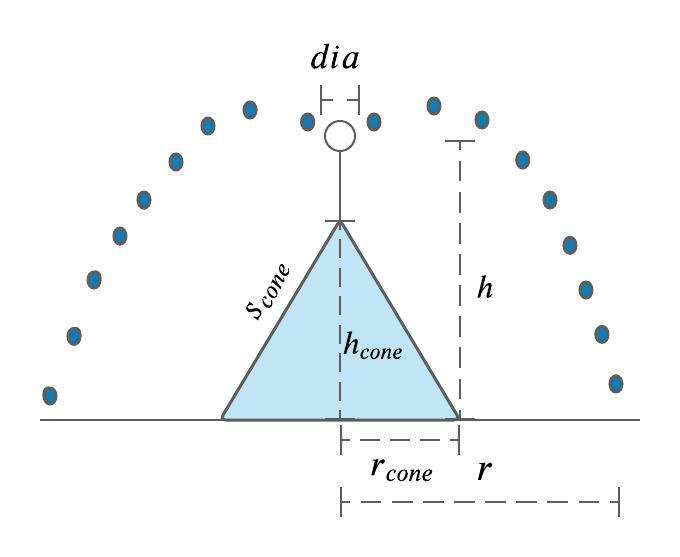
\includegraphics[width=12cm]{Figures/Fountain characteristics.jpeg}

\caption{Shape variables and fountain characteristics of the AIR. $r_{cone}$ is the radius, $h_{cone}$ is the
height and $s_{cone}$ is the slope of the AIR ice cone. $r$ is the spray radius, $dia$ is the aperture diameter
and $h$ is the fountain height}

\label{fig:fchar}
\end{figure*}

The fountain's height ($h$), aperture diameter ($dia$) and pressure loss ($P$) were related to its discharge
rate ($Q$) through the Bernoulli equation :

\begin{equation}
  \label{eqn:bernoulli}
  P_{i} + \rho_{water} \cdot g \cdot h_{i} + 1/2 \cdot \rho_{water} \cdot v_{i}^2 = P_{f} + \rho_{water} \cdot g
  \cdot h_{f} + 1/2 \cdot \rho_{water} \cdot v_{f}^2
\end{equation}

where $\rho_{water}$ is the density of water and $v$ is the velocity of the fountain water droplets. The
subscripts $i$ and $f$ refer to the initial and final states of the system. $v$ can be determined from the
discharge rate $Q$ through the mass conservation equation as 

\begin{equation}
	\label{eqn:dis}
 v = 4 \cdot Q/(\pi \cdot dia^2)
\end{equation}

Combining the Eqns. \ref{eqn:bernoulli} and \ref{eqn:dis}, we get the final discharge $Q_f$ after a height change
from $h_i$ to $h_f$ to be:

\begin{equation}
  \label{eqn:discharge}
  Q_f = \sqrt{Q_i^2 + 2 \cdot g \cdot (h_i-h_f) \cdot (\pi \cdot dia^2/4)^2}
\end{equation}

Traditional AIR construction often involves regular increase in fountain height in steps of 1 $m$. These events
can trigger fountain freezing events by reducing the pipeline discharge to zero.

Assuming that the water droplets have diameter equal to the fountain apertutre diameter and follow projectile
motion starting from a fountain height $h$ with a launch angle $\theta = 45 \degree$, we get the following
equation for the spray radius $r$:

\begin{equation}
  \label{eqn:radf}
  r = \frac{v \cdot(v + \sqrt{v^2 + 4hg)}}{2g}
\end{equation}

\section{Results}

\subsection{Estimation of fountain characteristics}

The influence of the fountain height increase event on the maximum discharge rate was used to determine the
fountain nozzle's aperture diameter. The maximum discharge rate of the scheduled fountain reduced from $Q_i$ =
13 $l/min$ to $Q_f$ = 11 $l/min$ when the fountain height was raised from  $h_i$ = 3 $m$ to $h_f$ = 4 $m$.
Inputting the corresponding values in Eqn. \ref{eqn:bernoulli}, we get the estimated fountain aperture diameter
($dia$) to be around 5 $mm$. 

The change in discharge rate observed upon removal of the fountain nozzle was used to determine the fountain
pressure loss. When the fountain nozzle was removed, the maximum discharge rate of the fountain was observed to
increase from $Q_{i}$ = 11 $l/min$ to $Q_{f}$ = 27 $l/min$. Using the fountain aperture diameter $d_i = 5 mm$,
the pipeline diameter $d_f = 19 mm$, $P_{f} = 0$ and $h_{i} = h_{f}$ in Eqn. \ref{eqn:bernoulli} we estimate the
pressure loss occurring due to the fountain nozzle to be equivalent to 4.3 meters of water head.

\subsection{Unscheduled discharge rate estimation}

The pressure loss of unscheduled fountain was determined by assuming a linear relationship of pressure loss with
aperture diameter. We use two observations to determine this linear relationship, namely, that the pressure loss
of the fountain was zero with a diameter of 19 $mm$ (fountain removal event) and that the scheduled fountain had
a pressure loss of 4.3 $m$ with an aperture diameter 5 $mm$. We estimate that for a constant height the pressure
decreases by 18 $mm$ for every 1 $mm$ increase in aperture diameter (see Fig. \ref{fig:fountains} (a)).

The fountain freezing event observation was used to determine the unscheduled fountain nozzle's aperture
diameter. The unscheduled fountain had a fountain freezing event at height 5.7 $m$. We assume that its discharge
rate was close to zero during this event.  The aperture diameter with the fountain freezing height closest to
5.7 $m$ is 7 $mm$ according to Eqn. \ref{eqn:bernoulli} as shown in Fig. \ref{fig:fountains} (b) . The
corresponding pressure loss of a fountain with 7 $mm$ diameter is 3.7 $m$ as shown in Fig. \ref{fig:fountains}
(a).

Fig. \ref{fig:fountains} (c) shows the unscheduled discharge rate estimated for the study period. The temporal
variation in the discharge rate is caused due to the the two height increase events on 23rd Dec and 12th
February that increased the height from 3.7 to 5.7 m respectively.

\begin{figure*}[t]
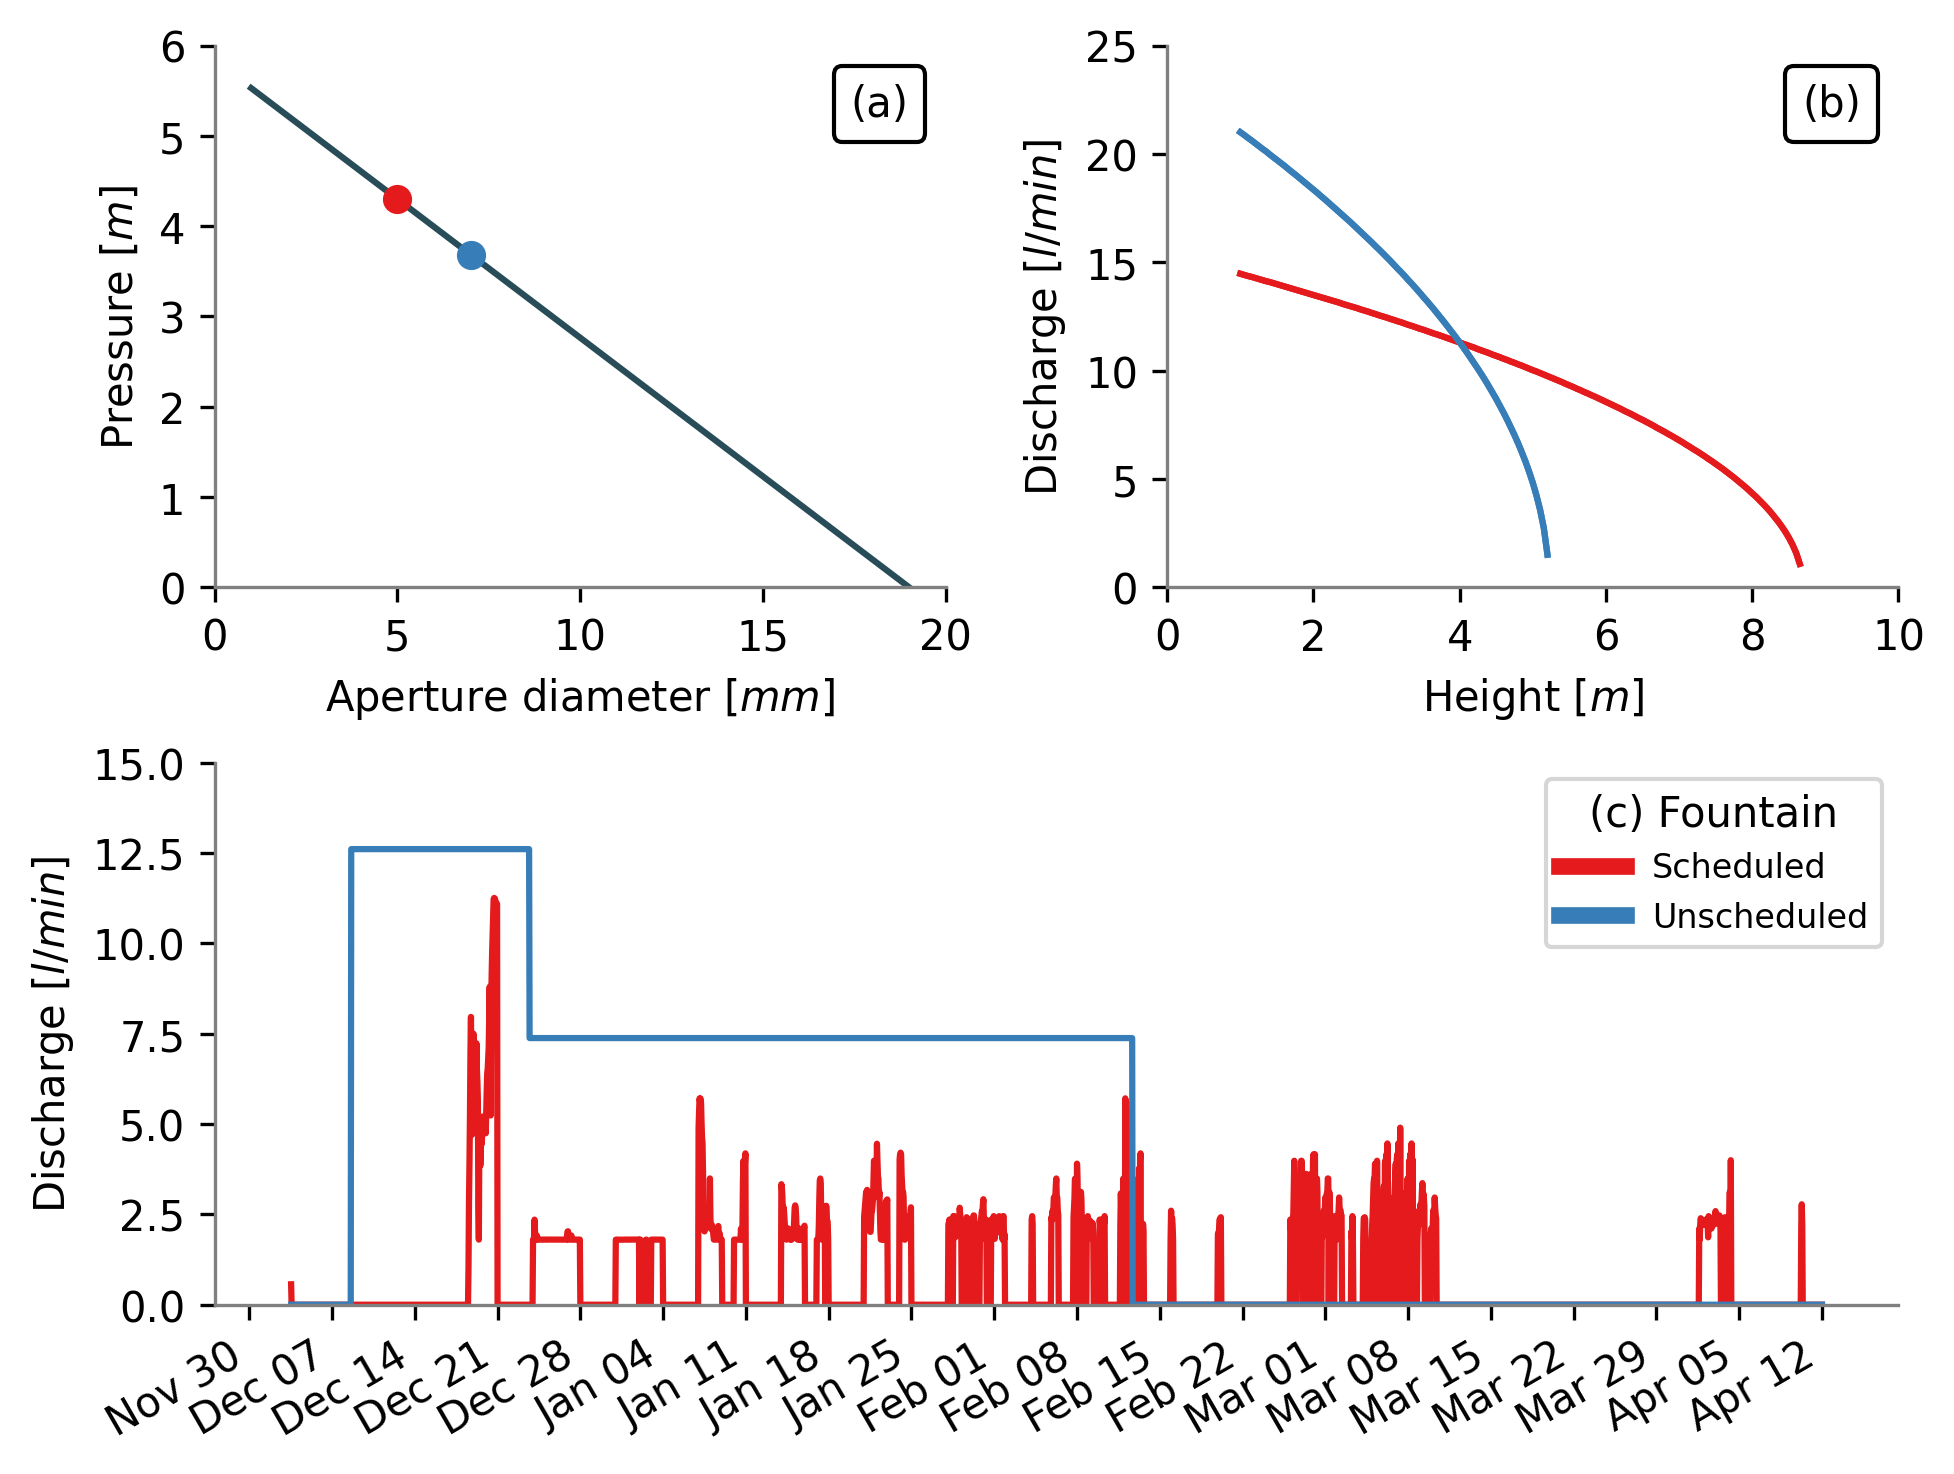
\includegraphics[width=12cm]{Figures/fountains.png}

\caption{ (a) Pressure loss as a linear function of aperture diameter for a constant fountain height and
  discharge rate. The corresponding values for the scheduled and unscheduled fountains are highlighted as red
  and blue dots respectively. (b) Discharge as a function of height for the scheduled (red curve) and the
  unscheduled (blue curve) fountain for a constant aperture diameter and pressure loss. (c) Discharge measured
  for the scheduled fountain (red curve) and estimated for the unscheduled fountain (blue curve) during the
study period.}

\label{fig:fountains}
\end{figure*}

\subsection{Scheduled discharge rate simulations}

We found that the MWE and MIV model versions estimated the freezing rate of the unscheduled fountain with a
correlation around 0.6 and a RMSE less than 0.6 $l/min$ and 1.6  $l/min$ respectively. The MIV scheduled
fountain overestimated the freezing rate 44 \% of the construction duration whereas the MWE scheduled fountain
underestimated the freezing rate 67 \% of the construction duration. Therefore, the MIV and MWE model forcings
were successful in prioritizing the maximum ice volume and water use efficiency metrics respectively.

\subsection{Model validation}

The volume estimation for the automated and traditional AIR had an RMSE of 13 $m^3$ and 5 $m^3$ with the drone
volume observations, respectively. This RMSE error is within 20 \% and 11 \% of the maximum volume of the
automated and the traditional AIR respectively. The estimated and measured AIR volumes are shown in Fig.
\ref{fig:validation}.  

\begin{figure*}[t] 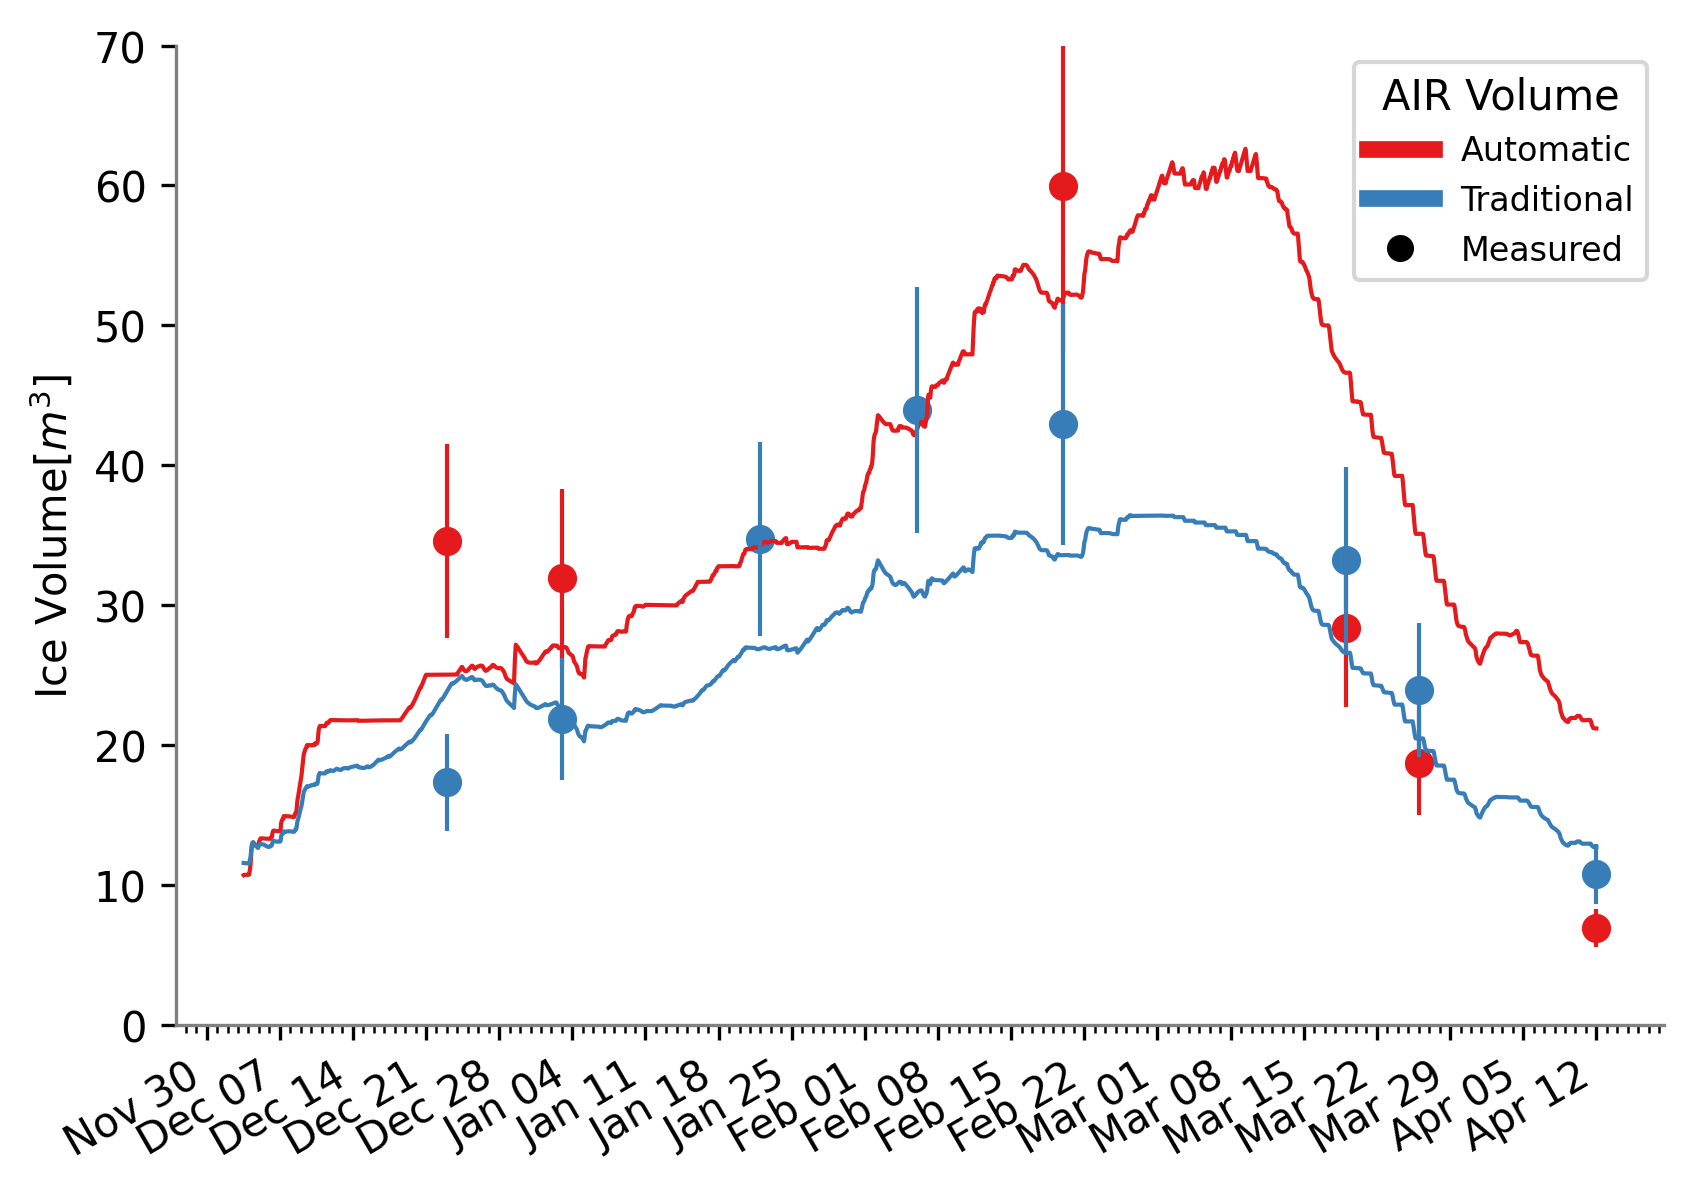
\includegraphics[width=12cm] {Figures/validation.png} \caption{Volume validation of the
scheduled and unscheduled fountain construction strategies.} \label{fig:validation} \end{figure*}

\subsection{Comparison of AIR construction strategies}

\begin{figure*}[t]
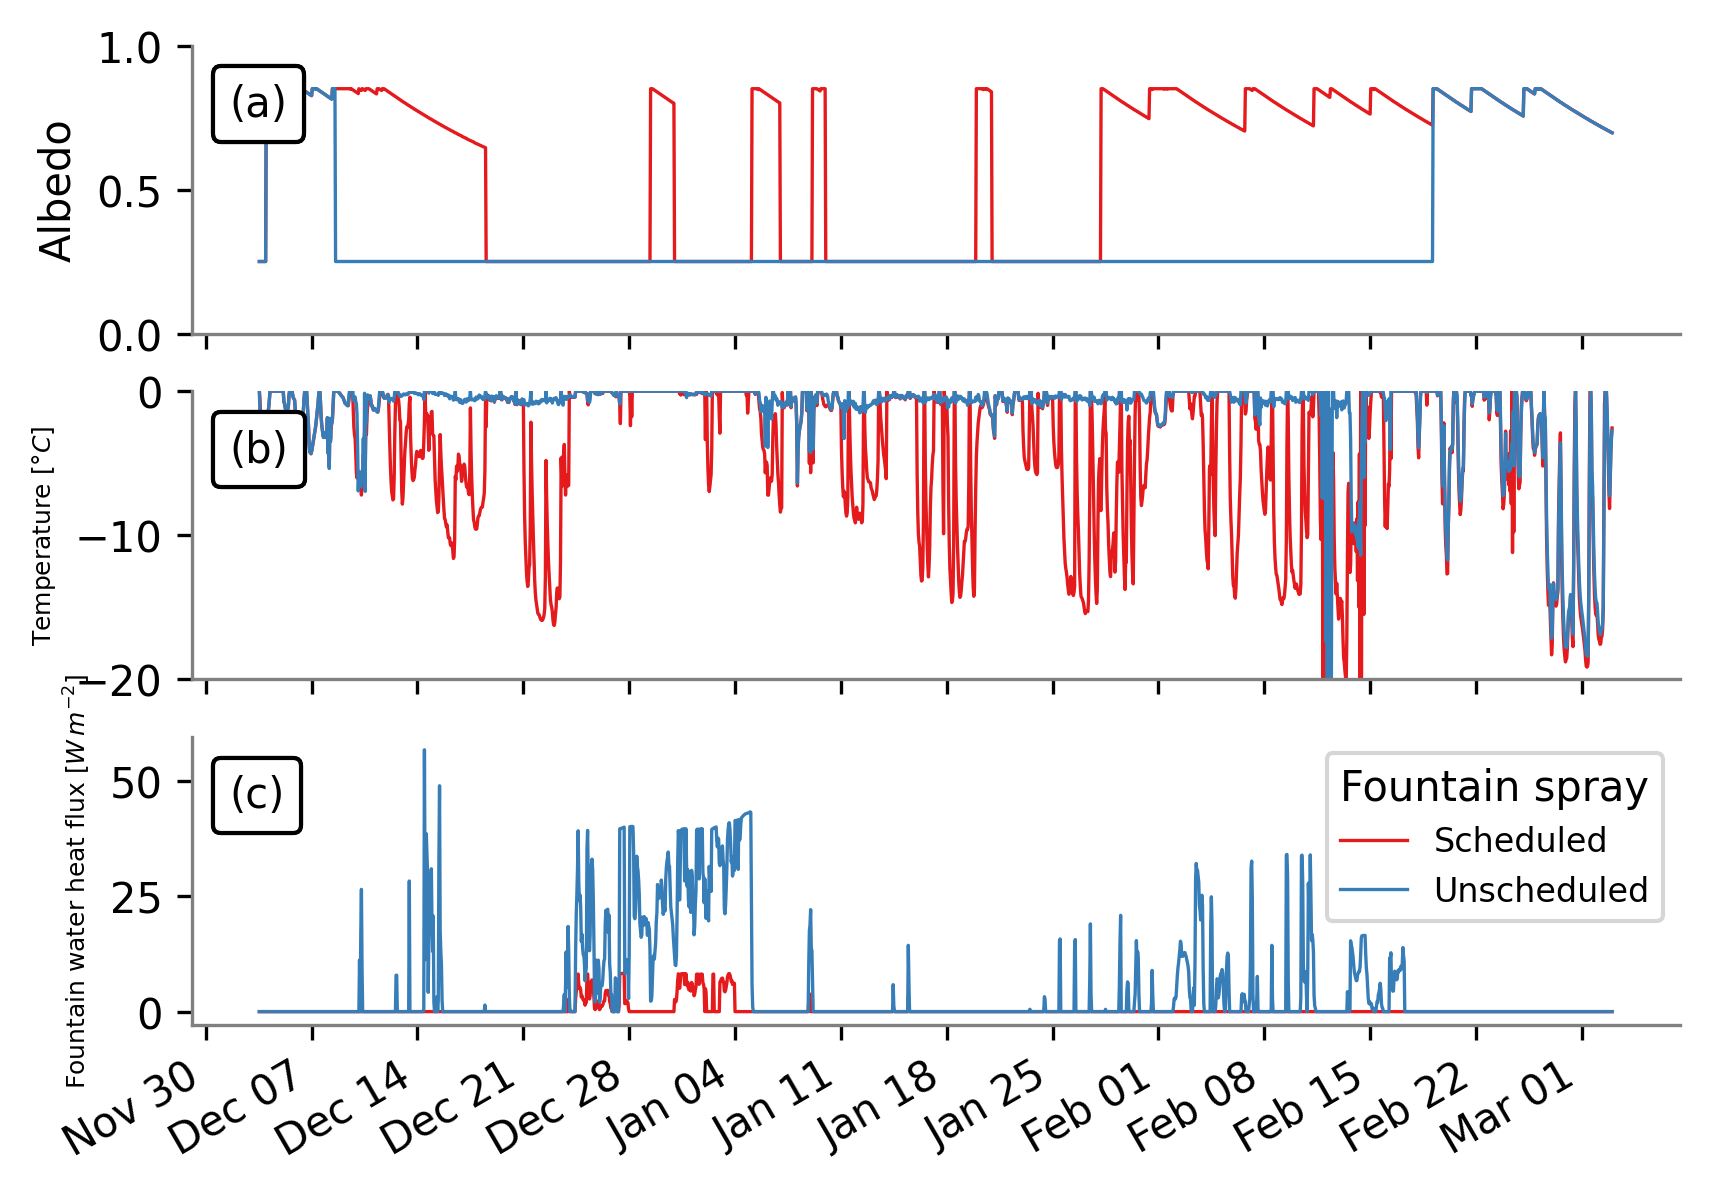
\includegraphics[width=12cm]{Figures/dis_processes.png}
\caption{(a) Surface albedo  and (b) fountain discharge heat flux showed significant variations between the two
  AIRS due to the differences in their discharge rates.}
\label{fig:dis_processes}
\end{figure*}

Table \ref{tab:mb} shows how the different fountain scheduling strategies influence the mass and energy balance
of the respective AIR. The difference between the fountain discharge input and fountain wastewater output of the
unscheduled and scheduled fountains was around an order of magnitude. This was expected since the unscheduled
fountain's discharge duration was 2 times higher than the scheduled fountain.

To understand how the different scheduling strategies influence the rest of the mass balance output, we discuss
the influence of fountain discharge on the surface mass and energy balance. During fountain spray, the AIR
surface (a) albedo dampens to ice albedo and (b) absorbs the heat energy of the fountain water droplets. These
two processes are the cause of the difference in the mass and energy balance distribution shown in Table
\ref{tab:mb}. The temporal variation of the magnitude of these processes are shown in Fig.
\ref{fig:dis_processes}. 

The overall impact of the radiation fluxes (long-wave and short-wave) and the turbulent fluxes (sensible and
latent) on the freezing and melting energies is determined from their respective energy turnover. The energy
turnover is calculated as the sum of energy fluxes in absolute values (see Table \ref{tab:mb}). 

There is a considerable difference in the contribution of the shortwave radiation due to the effect of process
(a). Even though the unscheduled fountain was active for a much longer duration, the frequent snowfall events
counteracted the albedo feedback of its fountain discharge. However, the albedo of the automated AIR was
significantly impacted by late fountain spray events particularly in the month of March and April as shown in
Fig. \ref{fig:dis_processes}.

Similarly, the fountain discharge heat flux for the traditional AIR was enhanced due to process (b). The higher
discharge quantity of the unscheduled fountains and its longer duration were responsible for the 10 fold
increase in its fountain discharge heat flux.


\begin{table}
	\centering
	\caption{Summary of the mass balance, energy balance, fountain and AIR characteristics estimated at the end of the respective
  simulation duration for the automated and the traditional AIRs}
	\label{tab:mb}
	\begin{tabular}{@{}|llllll|@{}}
		\toprule
		\textbf{}              & \textbf{Name}                   & \textbf{Symbol} & \textbf{Traditional} & \textbf{Automated} &
		\textbf{Units}                                                                                                       \\ \midrule
		\multicolumn{1}{|l|}{\multirow{3}{*}{\rotatebox[origin=c]{90}{Input}}}
		                       & Fountain discharge              & $M_F$           & \num{8.2e5}   & \num{1.4e5}     & $kg$  \\
		\multicolumn{1}{|l|}{} & Snowfall                        & $M_{ppt}$       & \num{1.1e4}   & \num{1.5e4}   & $kg$  \\
		\multicolumn{1}{|l|}{} & Deposition                      & $M_{dep}$       & \num{9.4e2}   & \num{1.2e3}     & $kg$  \\ \midrule
		\multicolumn{1}{|l|}{\multirow{4}{*}{\rotatebox[origin=c]{90}{Output}}}
		                       & Meltwater                       & $M_{water}$     & \num{2.9e4} & \num{4.2e4}   & $kg$  \\
		\multicolumn{1}{|l|}{} & Ice                             & $M_{ice}$       & \num{1.3e4} & \num{1.3e4}    & $kg$  \\
		\multicolumn{1}{|l|}{} & Sublimation                     & $M_{sub}$       & \num{2.6e3} & \num{3.0e3}     & $kg$  \\
		\multicolumn{1}{|l|}{} & Fountain wastewater             & $M_{waste}$     & \num{8.0e5} & \num{1.1e5}     & $kg$  \\ \midrule
		\multicolumn{1}{|l|}{\multirow{6}{*}{\rotatebox[origin=c]{90}{Energy Flux}}}

                           & Shortwave radiation             &  $q_{SW}$       & $29$  & $39$ & \% \\
		\multicolumn{1}{|l|}{} & Longwave radiation              &  $q_{LW}$       & $35$  & $34$ & \% \\
		\multicolumn{1}{|l|}{} & Sensible heat                   &  $q_{S}$        & $8$   & $8$ & \% \\
		\multicolumn{1}{|l|}{} & Latent heat                     &  $q_{L}$        & $17$  & $17$ & \% \\
		\multicolumn{1}{|l|}{} & Fountain discharge heat         &  $q_{F}$        & $10$  & $1$     & \% \\
		\multicolumn{1}{|l|}{} & Rain heat                       &  $q_{R}$        & $0$  & $0$     & \% \\
		\multicolumn{1}{|l|}{} & Ground heat                     &  $q_{G}$        & $1$   & $2$     & \% \\\midrule
		\multicolumn{1}{|l|}{\multirow{4}{*}{\rotatebox[origin=c]{90}{Fountain}}}

                           & Spray Radius                    &  $r$            & 4.8           & 4.1           & $m$ \\
		\multicolumn{1}{|l|}{} & Aperture Diameter               &  $dia$          & 5             & 7             & $mm$ \\
		\multicolumn{1}{|l|}{} & Pressure Loss                   &  $P$            & 4.3           & 3.7           & $m$ \\
		\multicolumn{1}{|l|}{} & Minimum discharge rate          &  $Q_{min}$      & 2           & N.A.          & $l/min$ \\\midrule
		\multicolumn{1}{|l|}{\multirow{2}{*}{\rotatebox[origin=c]{90}{AIR}}}

		                       & Maximum AIR Volume              &                 & 47            & 63            & $m^{3}$ \\
		\multicolumn{1}{|l|}{} & Water Use Efficiency            &                 & 4             & 31            & \% \\\midrule
	\end{tabular}
\end{table}


\section{Discussion}

\begin{figure*}[t]
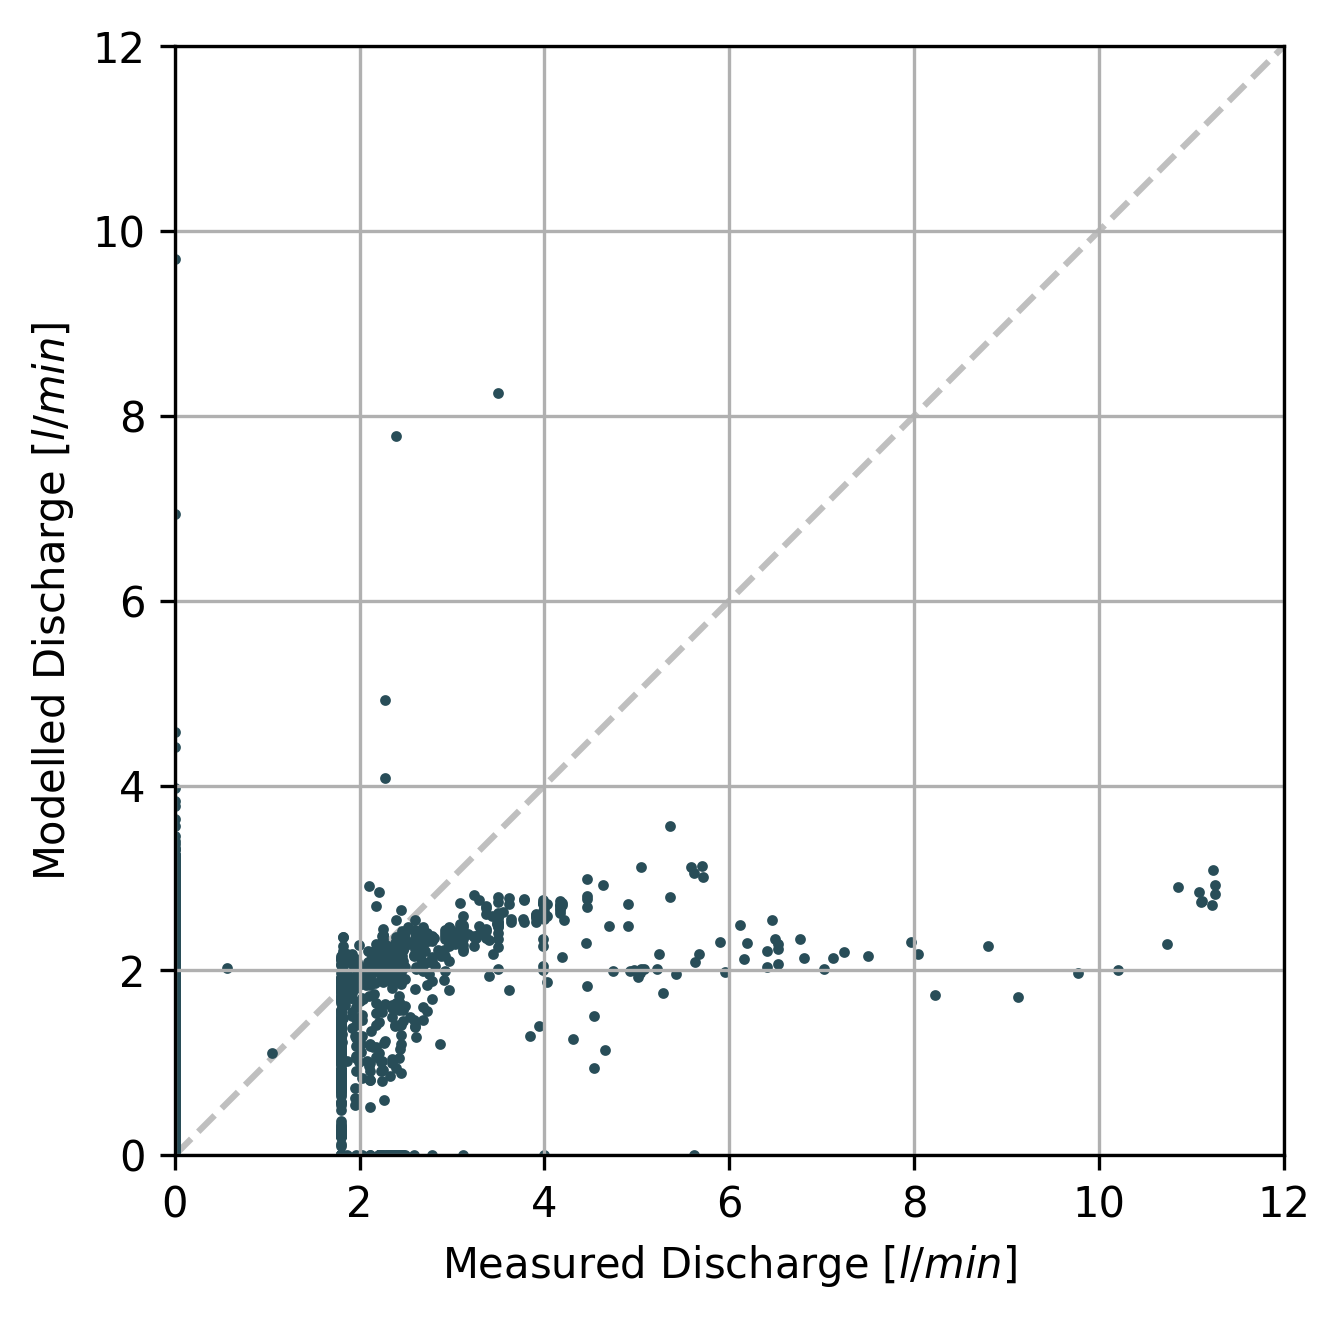
\includegraphics[width=8cm]{Figures/simvsreal2.png}

\caption{ Comparison of the discharge rate measured by the automation system and the discharge rate simulated by the MIV
model. }

\label{fig:simvsreal}
\end{figure*}

\subsection{Benefits of scheduling fountains}

The difference in water-use efficiency and maximum volume between unscheduled and scheduled fountains in the two
locations across two winters are presented in Fig. \ref{fig:wue}. Four experimental values (highlighted by
circles) are shown together with five simulated values (highlighted by squares).  The experimental values were
taken from the IN21 and CH21 AIRs studied in \citet{balasubramanianInfluenceMeteorologicalConditions2022} and
the CH22 AIR presented in this paper. 

\begin{figure*}[t]
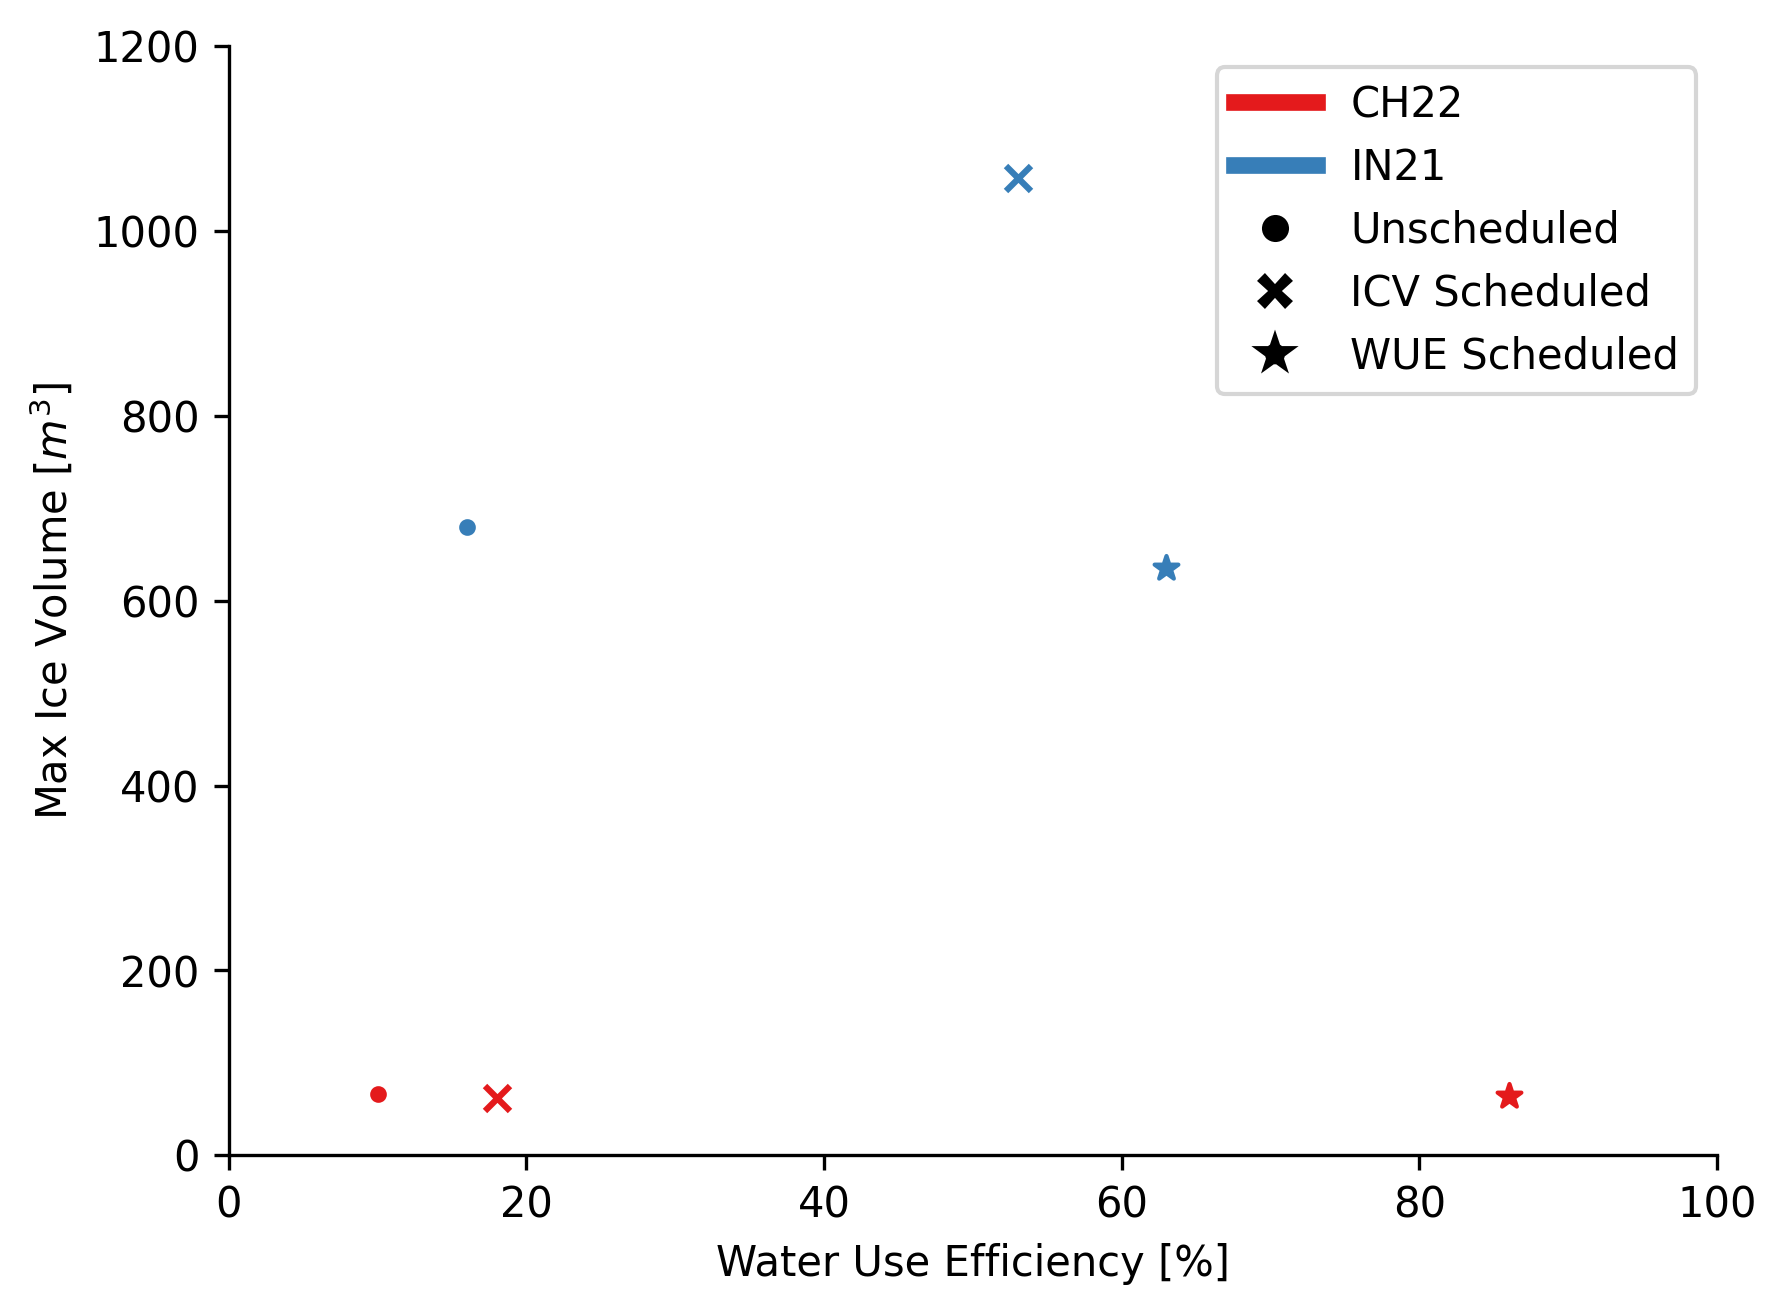
\includegraphics[width=\textwidth]{Figures/wue.png}

\caption{(a) The maximum volumes and water-use efficiency estimated for AIRs constructed in different locations
(represented by colours) with different fountain scheduling strategies (represented by symbols). Experimental
values are highlighted by circles and simulated values are highlighted by squares. (b) Comparison of
the unscheduled and scheduled fountain's discharge rates at the IN21 location.}

\label{fig:wue}
\end{figure*}

% \subsubsection{Higher water-use efficiency and maximum volume}

The water-use efficiency of all the unscheduled fountains are below 20 \%. In general, the water-use efficiency
increases more than two fold when the MIV or MWE fountain is used in both the locations.  

There is also considerable difference between the outputs of MWE and MIV fountains for each AIR. For CH21 AIR,
MWE fountain does not yield any ice formation whereas MIV fountain succeeds in increasing the water-use
efficiency three fold. For CH22 AIR, both experimental and simulated values of MIV fountains yield an increase
in water-use efficiency from 4 \% to around 31 \%. The MWE fountain succeeded in increasing the water-use
efficiency upto 2 times higher than the MIV fountain.

For the Swiss location, scheduled fountains yield better water-use efficiency but do not alter the maximum
volume obtained significantly. 

For the Indian location, the two kinds of scheduled fountains yield significantly different results when
compared to the unscheduled fountain. The MIV fountain achieved a 1.5 fold increase in the maximum volume and a
2 fold increase in the water-use efficiency. The MWE fountain had a water-use efficiency of 73 \% but its
maximum volume was lower than the unscheduled fountain. 

The discharge duration and the max discharge rate of these three fountains were responsible for these different
results (see Fig. \ref{fig:wue} (b)). The max discharge rate of the unscheduled fountain was more than twice
that of scheduled fountains resulting in a high water loss.  Fountain freezing events caused frequent
interruptions in the unscheduled discharge rate (see Fig. \ref{fig:wue} (b)). Therefore, the discharge duration
of the unscheduled fountain was much lower resulting in lower ice volumes. The MWE fountain underestimated the
freezing rate during the construction period and therefore produced much lower ice volumes compared to the
MIV fountain.

\subsection{Challenges of scheduling fountains}

\subsubsection{Determination of minimum discharge rate}

The value of minimum discharge rate determines the duration of the favourable weather windows and the risk of
fountain freezing events. Therefore, its accurate quatification is critical. The risk of a fountain freezing
event is inversely proporational to the spray radius the discharge rate produces. Therefore, minimum discharge
rate can be determined based on the minimum fountain spray radius desired. In the case of the CH22 experiment,
the minimum discharge rate of 2 $l/min$ corresponded to a spray radius of around 1 $m$.

\subsubsection{Determination of fountain spray radius}

To schedule fountains, one needs to estimate their spray radius accurately since the recommended discharge rate
is proportional to the square of the spray radius used.  Manual measurements of the fountain spray revealed a
maximum spray radius of just 3 m but drone measurements reveal a fountain spray radius of 4.8 m for the
scheduled fountain. This discrepancy could be caused by both wind drift of water droplets and refreezing events
across the boundary of the AIR. 

\conclusions

In this paper, an automated AIR construction strategy is presented and compared with a traditional strategy
using data collected in Guttannen, Switzerland and Gangles, India.

The main purpose of this study was to quantify the influence of different fountain designs and weather-sensitive
scheduling strategies on the water use efficiency and volumes of AIRs exposed to identical weather conditions.
We found that overwatering not just increased the fountain wastewater production but also enhanced the melting
rate of AIRs, mainly due to its surface albedo and fountain heat flux feedbacks. Furthermore, the freezing rate
of the scheduled fountain was also enhanced by its lower aperture diameter, which contributed to its higher
spray radius. As a consequence, the automated AIR was able to reduce its water consumption by 87 \% and increase
its maximum volume by 34\% compared to the traditional AIR.

Two different model forcings sensitive to the limited weather windows or water supply of a new location were
used to produce two types of recommended discharge rates favouring higher volumes and better water use
efficiencies, respectively. Nevertheless, these models were able to capture more than 44 \% of the freezing rate
variations produced by the full energy balance model. Simulations comparing scheduled and unscheduled fountains
show that up to a two fold increase in water use efficiency is possible without compromising on meltwater
production.

Fountain design is an important area where improvement is necessary since it can be used to increase AIR ice
volumes. If the scheduled fountain of the CH22 experiment was replaced with a fountain with a lower pressure
loss but with the same aperture diameter, the automated AIR would have produced more meltwater. Future research
must be devoted to engineer such fountains that create larger AIRs with user-desired shapes.

\appendix


\section{Model updates} \label{sec:Mod_updates}

In the previous version of the model \citep{balasubramanianInfluenceMeteorologicalConditions2022}, the fountain
water temperature ($T_F$) was estimated as a constant parameter. However, in reality, this is a poor
approximation. This is because the fountain water temperature and source water temperature differ due to the
temperature change caused by transit from the source to the  AIR surface. Therefore, we instead use measured
hourly ground temperature measurements to approximate water temperature for both the AIRs.

In the previous version of the model \citep{balasubramanianInfluenceMeteorologicalConditions2022}, fountain
discharge events were reset from surface albedo to ice albedo. However, this assumption limits the accuracy of
the model, especially, for the automated AIR where several fountain discharge events of short durations occur.
Therefore, we assumed that discharge events instead reduce the albedo decay rate ($\tau$) by a 
factor of $\frac{\alpha_{ice}}{\alpha_{snow}}$.

Additionally, both the AIRs experienced many precipitation events. Therefore, it was no longer accurate to
assume AIR density ($\rho_{cone}$) to be equal to ice density. We instead parameterised AIR density $\rho_{cone}$ as follows:

\begin{equation}
  \rho_{cone} = \frac{M_{F} + M_{dep} + M_{ppt}}{(M_{F} + M_{dep})/\rho_{ice} + M_{ppt}/\rho_{snow}}
\end{equation}

where $M_F$ is the cumulative mass of the fountain discharge; $M_{ppt}$ is the cumulative precipitation;
$M_{dep}$ is the cumulative accumulation through water vapour deposition; $\rho_{ice}$ is the ice density (917
$kg\,m^{-3}$) and $\rho_{snow}$ is the density of wet snow (300 $kg\,m^{-3}$) taken from
\cite{cuffeyPhysicsGlaciers2010} .

Rain events were not considered in the previous version of the model but they occur in our experiment. The
influence of rain events on the albedo and the energy balance was assumed to be similar to that of discharge
events. However, the water temperature of a rain event was assumed to be equal to the air temperature.
Accordingly, the heat flux generated due to a rain event was equal to:

\begin{equation}
  q_{R} = \frac{\Delta M_{ppt} \cdot c_{water} \cdot T_{a}}{\Delta t \cdot A_{cone}}
\end{equation}

\section{Model forcing based on water-use efficiency and maximum volume objectives} \label{sec:SEB}

The model complexity and data requirement \citep{balasubramanianInfluenceMeteorologicalConditions2022} were
reduced through assumptions that optimise for the ice volume or the water-use efficiency objectives. We define
the freezing rate and melting rate as the positive and negative mass change rate, respectively. Assumptions are
chosen, based on whether they overestimate/underestimate the freezing rate. HIV objective requires freezing rate
to be overestimated whereas water-use efficiency objective requires freezing rate to be underestimated. We
describe these two kinds of assumptions applied on each of the energy balance components below: 

\subsection{Surface Area $A_{cone}$ assumptions}

Determination of the surface area during the accumulation period is achieved by assuming a constant ice cone
radius equal to the fountain spray radius. The surface area scales the freezing rate of the AIR. Hence, for the
HIV objective, we assume the maximum possible slope of 1 for the ice cone or in other words $h_{cone} = r_{F}$.
Therefore, area is estimated as:  

\begin{equation} A_{cone} =\sqrt{2} \cdot \pi \cdot r_{F}^2  \end{equation}

Similarly, for the water-use efficiency objective, the area of the conical AIR is approximated to the area of
its circular base. Therefore, area is estimated as:

\begin{equation} A_{cone} =\pi \cdot r_{F}^2  \end{equation}

\subsection{Net shortwave radiation \texorpdfstring{$q_{SW}$}{Lg} assumptions}
\label{sec:SW}

The net shortwave radiation $q_{SW}$ is computed as follows:

\begin{equation} 
q_{SW} = (1- \alpha) \cdot ( SW_{direct} \cdot f_{cone} + SW_{diffuse})
\label{eqn:SW} 
\end{equation}

where $\alpha$ is the albedo value ; $SW_{direct}$ is the direct shortwave radiation; $SW_{diffuse}$ is the
diffuse shortwave radiation and $f_{cone}$ is the solar area fraction.

The data requirement was reduced by estimating the global shortwave radiation and pressure directly using the
location's coordinates and altitude through the solar radiation model described in
\citet{holmgrenPvlibPythonPython2018}. The algorithm used to estimate the clear-sky global radiation is
described in \citet{ineichenBroadbandSimplifiedVersion2008}.  

The diffuse and direct shortwave radiation is determined using the estimated global solar radiation as follows:

\begin{equation}
\begin{split}
  SW_{diffuse} &= cld \cdot SW_{global}\\
  SW_{direct} &= (1-cld) \cdot SW_{global}
\end{split}
\end{equation}

where $cld$ is the cloudiness factor. $cld$ is assumed to be 1 and 0 for the water-use efficiency and ice volume
objective respectively.

We ignore the variations in the albedo and assume it to be equal to snow albedo and ice albedo for the  ice
volume and water-use efficiency objective, respectively.

The solar area fraction $f_{cone}$ of the ice structure exposed to the direct shortwave radiation depends on the
shape considered. It is computed as

\begin{equation}
		f_{cone} =\frac{(0.5 \cdot r_{cone} \cdot h_{cone}) \cdot cos \theta_{sun} +(\pi \cdot
			{(r_{cone})}^2/2) \cdot sin \theta_{sun} }{\pi \cdot r_{cone} \cdot ({(r_{cone})}^2+{(h_{cone})}^2)^{1/2}}\\
\end{equation}

For the ice volume objective, since we assume the slope of the cone to be 1, $f_{cone}$ is determined as follows:

\begin{equation}
		f_{cone} =\frac{ cos \theta_{sun} + \pi \cdot sin \theta_{sun} }{2\sqrt{2} \cdot \pi }
\end{equation}

Similarly, for the water-use efficiency objective, since we assume the slope of the cone to be negligible, we get:

\begin{equation}
		f_{cone} =\frac{ sin \theta_{sun} }{2 }
\end{equation}

\subsection{Net Longwave radiation \texorpdfstring{$q_{LW}$}{Lg} assumptions} 

We assume $T_{ice} = 0 \degree C$ in order to determine outgoing longwave radiation. Since it is challenging to
constrain the minimum ice temperature, we maintain this assumption for both our objectives. However, in order to
estimate atmospheric emissivity, we again assume $cld$ to be 1 and 0 for the water-use efficiency and ice volume
objective respectively.

\subsection{Turbulent fluxes assumptions} \label{sec:Qs}

Turbulent fluxes estimation depend on the slope of the cone through the $\mu_{cone}$ parameter. As suggested 
by \citet{oerlemansBriefCommunicationGrowth2021}, we estimated this parameter as follows:

\begin{equation}
  \mu_{cone} =1 + s_{cone}/2
\end{equation}

Hence, the $\mu_{cone}$ parameter takes values of 1.5 and 1 for the ice volume and water-use efficiency
objective respectively.  Since turbulent fluxes impact both the freezing and the melting rates, this assumption
may not favor the corresponding objectives for certain sites.

\appendixtables   %% needs to be added in front of appendix tables

\begin{table}
  \caption{Free parameters in the model categorised as constant, model hyperparameters and weather 
  parameters with their respective values/ranges.}

	\label{tab:parameters}
	\begin{tabular}{lllll}
		\toprule

		\textbf{Constant Parameters}                       & \textbf{Symbol} & \textbf{Value} &
    \textbf{Unit} & \textbf{References} \\
    Van Karman constant & $\kappa$      & 0.4        &dimensionless & \citet{cuffeyPhysicsGlaciers2010}              \\
    Stefan Boltzmann constant & $\sigma$ & $\num{5.67 e-8} $& $W\, m^{-2}\, K^{-4}$ & \citet{cuffeyPhysicsGlaciers2010}\\
    Air pressure at sea level & $p_{0,a}$ & 1013 & $hPa$  & \citet{molgAblationAssociatedEnergy2004}\\
    Density of water & $\rho_{w}$ & 1000 & $kg\, m^{-3}$    & \citet{cuffeyPhysicsGlaciers2010}\\
    Density of ice & $\rho_{ice}$ & 917 & $kg\, m^{-3}$ & \citet{cuffeyPhysicsGlaciers2010}\\
    Density of air & $\rho_{a}$ &  1.29 & $kg\, m^{-3}$   & \citet{molgAblationAssociatedEnergy2004}\\
    Specific heat of water & $c_{w}$ & 4186 & $J\, kg^{-1}\,\degree C^{-1}$  & \citet{cuffeyPhysicsGlaciers2010}\\
    Specific heat of ice & $c_{ice}$ & 2097 & $J\, kg^{-1}\,\degree C^{-1}$ & \citet{cuffeyPhysicsGlaciers2010}\\
    Specific heat of air & $c_{a}$ & 1010 & $J\, kg^{-1}\,\degree C^{-1}$ & \citet{molgAblationAssociatedEnergy2004}\\
    Thermal conductivity of ice & $k_{ice}$ & 2.123  & $W\, m^{-1}\, K^{-1}$ & \citet{bonalesThermalConductivityIce2017} \\
    Latent Heat of Sublimation & $L_{s}$ & \num{2.848e6}  & $J\, kg^{-1}$ &   \citet{cuffeyPhysicsGlaciers2010}\\
    Latent Heat of Fusion & $L_{f}$ & \num{3.34e5} & $J\, kg^{-1}$ & \citet{cuffeyPhysicsGlaciers2010}\\
    Gravitational acceleration & $g$ & 9.81 & $m\, s^{-2}$ &\citet{cuffeyPhysicsGlaciers2010}\\
    Weather station height & $h_{AWS}$ & 2 & $m$ & assumed \\
    Model timestep                            & $\Delta t$            & $3600$           & $s$ & assumed \\\midrule

		\textbf{Model Hyperparameters} & \textbf{Symbol} & \textbf{Range} & \textbf{Unit} & \textbf{References} \\
    Surface layer thickness             & $\Delta x$            & $[\num{1e-2},\num{1e-1}]$           & $m$ & assumed
    \\\midrule
		\textbf{Weather Parameters} & \textbf{Symbol} & \textbf{Range} & \textbf{Unit} & \textbf{References} \\
    Ice Emissivity                      & $\epsilon_{ice}$      & $[0.95,0.99]$         & dimensionless & \citet{horiInsituMeasuredSpectral2006}             \\
    Surface Roughness                   & $z_0$                 & $[\num{1e-3},\num{5e-3}]$            & $m$  & \citet{brockMeasurementParameterizationAerodynamic2006}       \\
    Ice Albedo                          & $\alpha_{ice}$        & $[0.15,0.35]$         & dimensionless  &
    \citet{steinerModellingIcecliffBackwasting2015};            \\
    & &    &  & \citet{zollesRobustUncertaintyAssessment2019}      \\
    Snow Albedo                         & $\alpha_{snow}$       & $[0.8,0.9]$        & dimensionless  & \citet{zollesRobustUncertaintyAssessment2019}              \\
    Precipitation Temperature threshold & $T_{ppt}$             & $[0,2]$            & $\degree C$& \citet{shichangResponseZhadangGlacier2010}  \\
    Albedo Decay Rate                   & $\tau$                & $[10,22]$           & $days$ &
    \citet{schmidtImportanceAccurateGlacier2017};      \\
    & &    &  & \citet{oerlemansYearRecordGlobal1998}      \\\midrule
	\end{tabular}
\end{table}
\clearpage


\noappendix 

\bibliographystyle{copernicus}
\bibliography{zot_refs.bib}

\end{document}
